\section{Independent execution and fresh confirmation}
Construction and conventional challenge were assigned to separate workstreams. The conventional implementation received the same event contract, input information and acceptance conditions. It used current AI assistance, direct event-history logic and the same free verification toolchain. It was not deliberately limited to an inferior model or a slower programming language while the candidate received hardware tools.

The main implementation, oracle, comparator and verifier were frozen before an independent entropy seed was selected. Confirmation then generated 24 fresh specifications, each with 32 traces of 256 ticks. The successor received its own source freeze and seed. This separation prevents the successor's new grammar from silently enlarging the predecessor's accepted scope.

\begin{table}[htbp]
\centering\small
\begin{tabular}{L{0.48\textwidth}rr}
\toprule Check & Main instrument & Successor network\\
\midrule
Fresh specifications / networks & 24 & 6\\
Fresh traces passed & 768 / 768 & 48 / 48\\
Logical ticks & 196,608 & 6,144\\
Positive output decisions & 630 & 62\\
Directed cases through actual RTL & 52 & 10\\
Invalid requests rejected & 14 & 9\\
Bounded equivalence checks & 28 & 12\\
Recorded proof depths & 8--22 & 16--34\\
Conventional functional comparison & Tie & Tie\\
Identical-artifact library comparison & Not a main claim & Tie\\
\bottomrule
\end{tabular}
\caption{Executed confirmation. The 491,520 main predicate-tick decisions include multiple predicates per input tick. Directed cases and proof obligations supplement random traces; they do not convert finite coverage into universal physical validation.}
\end{table}

\subsection{A failure that improved the evidence}
The first development run reported apparent one-tick delays in 18 of 32 traces. Both RTL implementations agreed with each other, and bounded equivalence passed. Investigation isolated a CXXRTL driver error: it read combinational outputs immediately after committing state, before a same-clock settling evaluation. The original driver and all failed observations remain preserved. The driver was corrected before freeze, without adding a clock edge, changing the product, or relaxing acceptance. Fresh confirmation used the corrected frozen harness.

This failure matters because agreement between two implementations can conceal a shared observation error. Independent mathematical models and explicit known-answer cases made the discrepancy visible. The final record includes the failure, diagnosis, correction and source hashes; it does not replace the first run with a success-only history.

\subsection{The comparator won an important performance test}
Across the fresh main cases, the EventWeaver Python model took 12.482 seconds, the conventional history model 0.276 seconds, and the offline oracle 0.181 seconds. The candidate Python model was approximately 45 times slower than the conventional model. Paired actual-RTL replay took 0.677 seconds, but that combined replay is not an isolated hardware throughput comparison.

The outcome supports functional correctness and a useful generated design pack. It defeats a broad claim that the prefix model is faster or that this agent-built representation is inherently superior. It also recommends using the simpler conventional model for software-only analysis when it meets the buyer's need. An RTL buyer may still value the complete pack, but that commercial claim must survive the price of the competent alternative.

\subsection{What is necessary for the outcome?}
The proposed transformational kernel is \emph{bounded temporal composition}: independent sequence windows, an inclusive veto interval that remains open until the decision deadline, and a decided event that can become a later instrument's input. These functions are exercised by the offered design pack. Their necessity for a selected contract must be distinguished from the necessity of our implementation, scientific novelty, or a newly viable business.

We therefore declared a separate, postconfirmation ablation protocol. Six explicit traces, the exact operator removals, the expected outputs, the comparison methods and the stopping rule were frozen at 14:19:23 UTC on 28 October 2026, before the ablation run. The retained main compiler, successor, independent conventional implementations, oracle and verifiers were checked against their recorded source hashes before and after execution; all remained unchanged. This extension does not enlarge the original fresh-confirmation sample.

The first mutation accepts an anchor irreversibly at its earliest valid C event, without waiting for future vetoes. The second pools all declared A channels, all B channels, all C channels and all veto channels across groups while retaining each predicate's own lag bounds. The third disconnects every virtual event by setting it to zero, preserving raw inputs and stage logic. Each mutation was executed both as a Python model and as generated RTL evaluated through Yosys CXXRTL. The full implementation was also compared with the independent oracle and conventional RTL on exactly the same traces.

\begin{table}[htbp]
\centering\small
\begin{tabular}{L{0.35\textwidth}L{0.25\textwidth}L{0.25\textwidth}}
\toprule Predeclared fixture & Full contract & Operator removed\\
\midrule
Late veto at tick 7 & No output & $0@2$ (false acceptance)\\
Same sequence, no veto & $0@7$ & $0@2$ (wrong time)\\
Events drawn from different groups & No output & $0@7,\;1@8$\\
Valid independent groups & $0@7,\;1@8$ & $0@7,\;1@8$\\
Virtual event activates second predicate & $0@8,\;1@14$ & $0@8$ only\\
Raw-stage control & $0@8$ & $0@8$\\
\bottomrule
\end{tabular}
\caption{Kernel counterfactuals. The notation $j@t$ means output bit $j$ at zero-based logical tick $t$. All six fixtures and 88 ticks matched their predeclared full and mutated outputs in executable models and actual RTL. The no-veto control preserves the existence of a match but reveals the early-accept mutation's changed decision time. No unexpected error occurred.}
\end{table}

\textbf{Removing our compiler did not remove the outcome.} Substituting the independently implemented conventional history-formula RTL, including the conventional successor network, preserved every result in all six fixtures. This counterfactual defeats a claim that EventWeaver itself was necessary for these outcomes. Temporal composition is a functional requirement of the selected contracts; EventWeaver is one implemented means of satisfying it. Existing conventional software and custom digital logic remain strong alternatives.

The result is therefore a tested construction with a necessary \emph{semantic} kernel, not an earned claim of exclusive transformational capability. The fixtures were deliberately chosen to expose the specified removals. They are not a blinded causal experiment on agent skill, a random estimate of field failure, or evidence that current frontier intelligence uniquely made the commercial opportunity feasible. Nor does an ablation establish customer willingness to pay. Full traces, source integrity records, generated mutant RTL and discrepancies are retained in \texttt{protocol/kernel\_ablation\_v1.json}, \texttt{protocol/kernel\_ablation\_freeze.json}, and \texttt{results/kernel\_ablation.json}.


\subsection{Independence and its limits}
The verifier and conventional code were separately authored rather than copied from the candidate. The ledger auditor imports neither the business simulator nor its accounting helpers. Nevertheless, these are separate AI-assisted workstreams in one campaign, with shared model-family risks. They are not a blinded human laboratory review, an independent customer acceptance, or a formal proof of every implementation layer. No human-specialist advantage is inferred from their agreement.

\section{The complete commercial offering}
\subsection{Scope that can be sold honestly}
The offering is a supported functional design pack for a bounded event contract. It contains validated specifications, generated source, reference behavior, independent acceptance evidence and limited support. The published compiler can be reused freely; the selected US\$1,200 fee is for service and accountable delivery, not an invented exclusive license over public source.

Qualification requires an existing digitized event interface, a request inside the grammar, a named acceptance authority, an actual need beyond installed functions, and a budget that survives comparison with internal/current-AI work. Requests for analog timing, vendor-link integration, safety-critical certification, unlimited predicates or unsupported timestamp semantics are refused or require a separate study. The commercial simulator never makes those missing capabilities succeed behind the scenes.

The modeled contract uses a 40\% refundable deposit, restricted until acceptance. The balance is due 60 days after acceptance, with modeled procurement and payment delays. A 45-day warranty permits repair, invoice credit and cash refunds. A 42-day delivery deadline applies to the contract, including pool formation and correction. Source and evidence are supplied under the declared rights; later revalidation is a separate US\$450 renewal service, chosen only when buyer utility and seller contribution justify it.

These are research contract terms rather than advice about enforceability in a particular jurisdiction. In particular, a buyer who has received source may strategically withhold the balance if enforcement, reputation and continuing-support incentives are absent. That payment-stage deviation is tested explicitly.

\subsection{Acquisition through exit}
The acquisition window lasts 180 days. The base assumptions begin with 180 scoped prospects, an 18\% inquiry probability, and 62\% qualification among inquiries. Marketing, failed qualification, quotations, negotiations and procurement refusals all consume resources. The proposal does not assume an unlimited queue of willing buyers.

The event simulation then executes contracting, restricted deposit custody, capacity/funding admission, implementation, initial acceptance or refusal, bounded correction, final acceptance or refund, support, warranty, collection or default, renewal quotation, renewal acceptance or refusal, and exit. Administration continues during runoff. The allowed horizon is 730 days; the latest base obligation occurs by day 450. No new intake continues indefinitely to conceal a losing first campaign.

Renewals have a narrower modeled lifecycle: after the utility and procurement gates, the simulator assumes accepted revalidation and full collection. It does not add a second technical-failure, correction, warranty or default cycle. This optimistic renewal assumption does not rescue the losing policy; it limits any claim that all repeat-delivery risks were tested.

One illustrative history was selected \emph{after} confirmation to show lifecycle behavior; it is not representative evidence chosen to optimize the result. In seed 700587, buyer B0034 negotiated US\$1,127.83, paid a US\$451.13 restricted deposit on day 18, initially refused the pack on day 20, accepted a correction under the unchanged contract on day 21, received support, and paid the US\$676.70 balance on day 129. The warranty closed on day 66 and the buyer did not renew. The same history includes defaults and full warranty refunds.

Buyer B0018 illustrates why acceptance and collection must remain distinct. A full warranty refund credited the remaining US\$688.96 receivable and returned the US\$459.31 already released deposit. Its later collection event simply closed a zero invoice balance; it was not another receipt. Buyer B0008 defaulted on US\$670.07, which remained a bad-debt cost. Dollar ledgers, rather than lifecycle event counts, determine revenue and cash.

\subsection{Buyer objectives, information and alternatives}
For buyer $i$ and alternative $a$, the model evaluates
\begin{equation}
U_i(a)=q_a V_i-p_a-w_i h_{ia}-\tau_i d_{ia}-T_{ia}-R_{ia},\label{eq:utility}
\end{equation}
where $V_i$ is the assumed value of a successful digital outcome, $q_a$ a belief about success, $p_a$ the price, $h_{ia}$ internal effort, $d_{ia}$ delay, $T_{ia}$ trust/onboarding burden, and $R_{ia}$ reuse-rights or setup burden. Buyers choose among the offering, a competitor, internal current-AI-assisted engineering, free tooling, waiting, and doing nothing. The last alternative has utility zero.

Gross value has a modeled median of US\$6,500, but this does not set the selling price. The strongest feasible outside utility limits the buyer's reservation price. Internal work uses six to sixteen design hours plus four to eight review hours; competitor quotes range from US\$1,500 to US\$3,300 before response factors. Both are explicit estimates for this small digital scope, not prices for a complete optical instrument. Supplier labor is anchored to public wage data and then increased to an assumed US\$135 per hour for specialist/business cost.\cite{bls,ecec}

The buyer privately knows its modeled value and outside cost and submits a bounded counter-bid. The seller observes that bid and its own expected incremental obligation, not the buyer's hidden reservation price. It refuses a bid below the cost gate or a contract beyond available capital commitments. This is a specified bargaining heuristic, not an incentive-compatibility theorem. Logged utilities, bids, prices and decisions allow an independent auditor to reconstruct the choices.

Modeled participation and a positive utility value are not independent willingness-to-pay evidence. They say what follows from the stated assumptions. The commercial gate remains actual buyer evidence.

\section{Inventing the arrangement, then testing its incentives}
\subsection{Three arrangements and a bounded price search}
Development compared three arrangements at posted fees of US\$1,200, 1,800, 2,400, 3,000 and 3,600. Each policy used 96 development seeds before the selection was frozen.

\textbf{Bespoke service} supplies more seller construction effort and less buyer setup. \textbf{Three-order pooling} shares a validation batch and requires nonexclusive core rights, explicit coordination, and a 28-day formation window. Unformed groups receive deposit refunds. \textbf{Supported library} uses retained source with fewer seller construction hours and more buyer-side setup. The buyer's extra work remains in Equation~\ref{eq:utility}; it is not silently moved out of the comparison.

Pooling creates a potential gain by avoiding repeated core validation. It also creates waiting, coordination, withdrawal and correlated-defect costs. Each participant must prefer the pooled outcome to its own best alternative. A buyer who will not share reuse rights pays the opportunity cost or chooses another route. Generic-core benefits can be copied by competitors, so the same pooled arrangement is available in the conventional strategic comparison.

All 15 development policies lost full-project money. The least-loss policy was the supported library at US\$1,200. It was frozen for research confirmation, not approved for launch. The option \emph{do not launch} has zero incremental project profit and dominates those launch policies under their development assumptions.

\begin{figure}[htbp]
\centering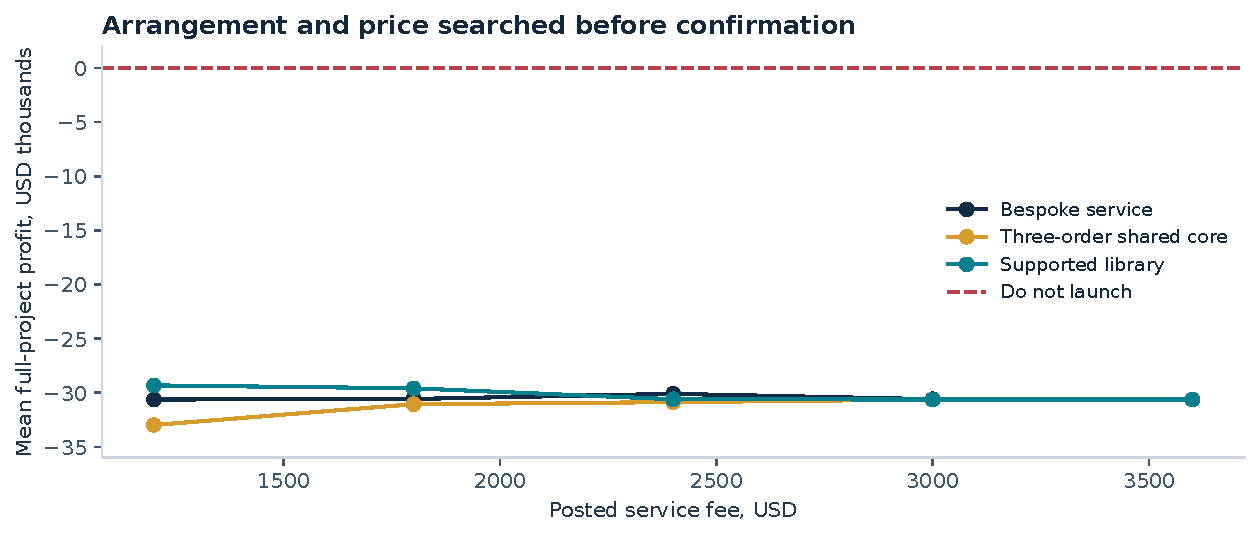
\includegraphics[width=\textwidth]{figures/development_policies.pdf}
\caption{Bounded price and arrangement search before confirmation. The horizontal zero-profit line is the no-launch outside action. A price that loses fewer dollars is not a commercially viable optimum.}
\end{figure}

\subsection{Competition and strategic behavior}
The lifecycle model includes a competitor price reduction, identical public-library access, and a conditional AI-improvement scenario for both seller and rivals. It does not assume that frontier progress belongs exclusively to this enterprise. Supplier quotes above a fixed US\$180-per-hour reservation are refused; capacity and rate shocks can therefore reduce activity rather than magically increase prices buyers will pay.

A separate finite price game makes the strategic issue explicit. Four thousand synthetic buyer types define a distribution of outside options; two firms post prices on a US\$900--3,000 grid and may decline entry. Both receive the same cost reduction when shared-core delivery is available. The entrant bears US\$23,000 of initial research construction; the incumbent's incremental fixed entry cost is zero. These are stylized assumptions, not an estimated market equilibrium.

Conditional on both firms remaining active, the individual-delivery game has two pure equilibria, at entrant/rival prices US\$900/1,200 and US\$1,200/1,500. Entrant profits remain negative. Allowing entry refusal yields no entry by the new firm and a US\$2,100 incumbent price on this finite grid. A shared-core cost reduction available to both does not change the no-entry conclusion. A bounded-rational logit response check also concentrates on exit. Independent reconstruction verified all 324 payoff cells and the reported best-response sets.

The game cannot identify unknown demand, customer value or enforcement costs. Its purpose is to test whether a claimed arrangement gain survives strategic access by rivals. It provides no reason to turn an unsupported demand assumption into a fact.

\subsection{The collection subgame and loss-leading claims}
After final source delivery, an opportunistic buyer may save the unpaid balance by defaulting. Compliance requires the expected enforcement, reputation or lost-support cost to exceed that saving. With a hypothetical US\$1,140 fee and a 40\% deposit, US\$684 remains exposed. The simulator's normal collection behavior is an assumption; the no-recourse stress defaults every postdelivery balance. Inspection-compatible escrow or payment before final-source handoff might improve incentives, but would change the contract and buyer participation and therefore requires a new frozen study.

The campaign also rejects an unsupported loss-leader argument. There is no observed downstream order book that can justify today's loss. Successor value is not booked as revenue, an asset uplift, or a second source of funding. The US\$4,100 research extension is charged once. A milestone may rationally lose money when a bounded, independently evidenced downstream benefit exceeds that loss; no such evidence was established here.

\section{Closing costs, cash and uncertainty}
\subsection{What the complete bill contains}
The full campaign includes discovery, failed attempts, core construction, independent verification, tools/data/compute, estimated inference, contract design, artifact extraction, the successor research option, acquisition, qualification, quotation, procurement, delivery, correction, support, common repair, warranty, bad debt, renewals, administration and financing. Shared construction is allocated once. The modeled US\$23,000 startup bill includes US\$4,100 for succession; acquisition-window fixed overhead adds US\$2,700. Later runoff administration is charged separately.

The selected policy uses three seller delivery hours per order, plus explicit qualification, support, repair and renewal work. It reserves eight additional delivery-capacity hours per order for obligations. That reserve is a conservative aggregate scheduling proxy; it is not a verified weekly support service level. Sales capacity is separately limited. Fixed research labor is charged in startup costs and is not misrepresented as measured human time.

\begin{table}[htbp]
\centering\small
\begin{tabular}{L{0.55\textwidth}r}
\toprule Fresh base result, 1,024 histories & Mean\\
\midrule
Accepted initial design packs & 7.94\\
Net recognized revenue & US\$9,024\\
Net customer cash after refunds and defaults & US\$8,836\\
Complete project expense & US\$38,653\\
Operating contribution before fixed costs and financing & US\$\(-3,928\)\\
Full-project profit & US\$\(-29,628\)\\
Return on total cost, ratio of means & \(-76.7\%\)\\
Mean unrestricted capital required & US\$32,111\\
95th percentile unrestricted capital required & US\$36,496\\
Mean variable human service hours & 72.81\\
Variable service hours per accepted outcome & 9.17\\
Modeled interventions per accepted outcome & 1.19\\
\bottomrule
\end{tabular}
\caption{Recognition, collections, operating contribution, full-project profit and capital are distinct. Human hours and interventions are explicit commercial assumptions; technical trace counts and tool runtimes are executed measurements.}
\end{table}

The average modeled buyer benefit conditional on participating histories is approximately US\$359 before realized outcomes, relative to the best modeled outside alternative. That is an output of assumed private values and delays, not measured customer savings. The selected service can benefit some modeled buyers while the enterprise loses after acquisition and fixed costs.

\begin{figure}[htbp]
\centering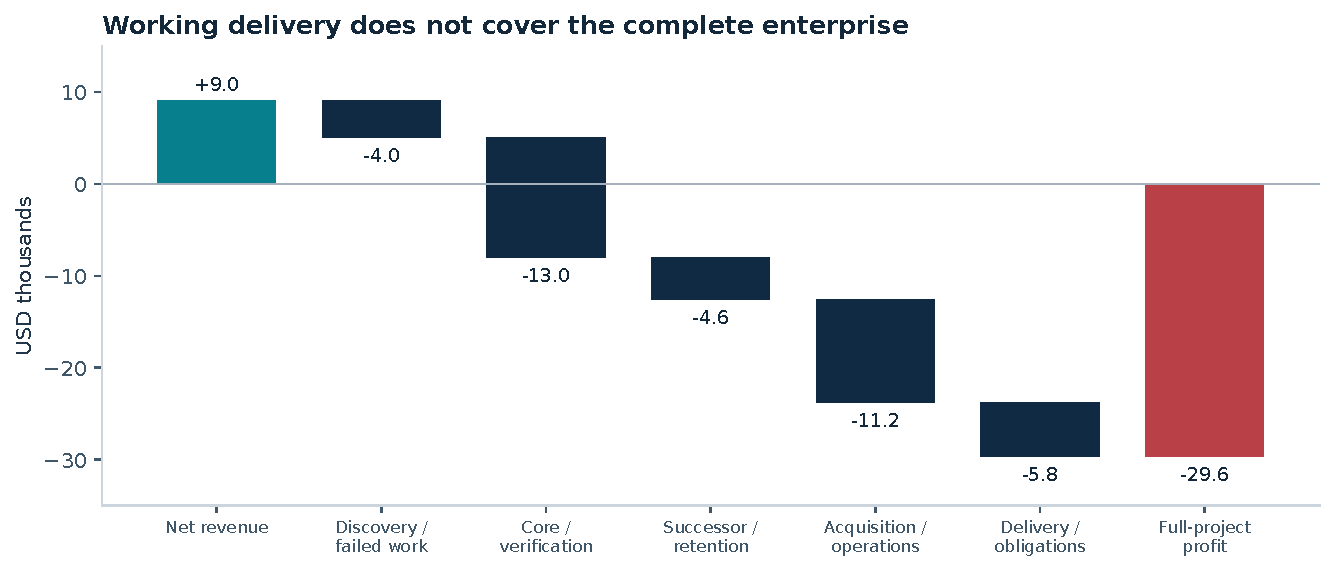
\includegraphics[width=\textwidth]{figures/economics_waterfall.pdf}
\caption{Complete-cost bridge for the frozen base policy. Operating losses remain even before the fixed research bill. Artifact retention and successor development are visible costs.}
\end{figure}

\subsection{Accounting and financing}
The journal uses integer cents and double-entry postings. A deposit debits restricted cash and credits a liability; it is not revenue or available working capital. Acceptance recognizes a receivable and revenue, applies the deposit against that receivable, and releases only the corresponding restricted cash. Collection exchanges receivables for cash without recognizing revenue again. Warranty first credits unpaid receivables and then refunds already collected cash. Defaults are bad debt, not invisible missing receipts.

The policy starts with US\$45,000 equity and a US\$15,000 credit ceiling at a 12\% annual rate. Contract admission uses recorded commitments and excludes refundable deposits. The reported required capital is the peak unrestricted deficit before financing, not hindsight used to approve contracts. The model permits an explicit emergency-equity requirement to register a funding failure; it does not turn such a requirement into successful free capital.

In base confirmation, no emergency injection or debt draw was required, and all modeled obligations settled. The broader stress campaign contains seven terminal insolvencies: one no-recourse history retains US\$2,524.62 of debt, and six high-demand histories retain US\$6,285.11 in aggregate across separate histories. These liabilities are not forgiven. Customer deposits, receivables and refunds close, but universal financing closure is not claimed. Unpaid debt is measured at each terminal date; later interest, creditor recovery and insolvency resolution are not simulated.

\subsection{Risk is conditional on the model}
Every base history lost money. The base 5th--95th percentile profit interval is US\$\(-34,181\) to US\$\(-26,599\); the mean of the worst five percent is US\$\(-36,449\). The Monte Carlo standard error of mean profit is about US\$76. The conditional 95\% Wilson interval for the sampled loss probability is 99.626\%--100\%.

That narrow interval quantifies sampling precision \emph{inside this model}. It does not measure real-world certainty about demand, buyer value, scope fit, support burden or competitor behavior. The cash-shortfall estimate is zero in the base sample, with a sampling upper bound of about 0.374\%, under the stated capital policy. It is not a promise that an actual enterprise needs no contingency capital.

\begin{figure}[htbp]
\centering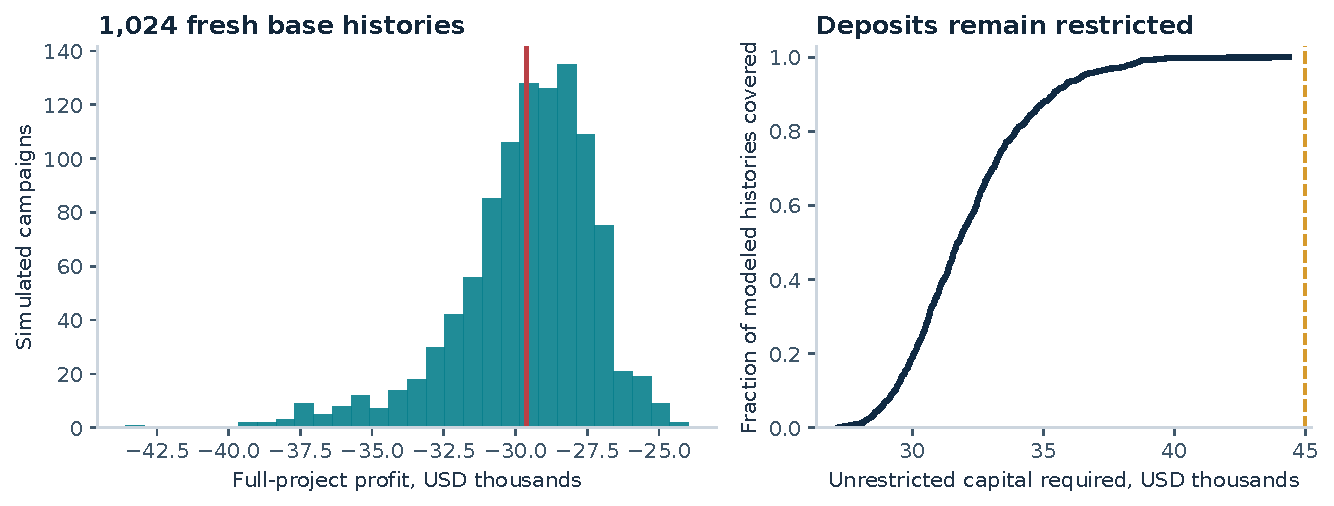
\includegraphics[width=\textwidth]{figures/uncertainty_cash.pdf}
\caption{Profit dispersion and capital coverage within the frozen base model. The dashed capital line marks US\$45,000 equity; refundable deposits are excluded. Model uncertainty is broader than these Monte Carlo distributions.}
\end{figure}

\begin{table}[htbp]
\centering\small
\begin{tabular}{L{0.57\textwidth}rr}
\toprule Conditional scenario, 1,024 histories each & Mean profit (US\$) & Accepted packs\\
\midrule
Base & \(-29,628\) & 7.94\\
Competitor price response & \(-30,410\) & 3.72\\
Weak demand & \(-28,305\) & 3.91\\
Supplier cost/capacity shock & \(-32,636\) & 0.79\\
Slow payment and more defaults & \(-30,195\) & 7.94\\
Correlated downturn & \(-30,397\) & 1.06\\
Identical free library & \(-30,767\) & 0.00\\
Conditional AI improvement for all firms & \(-30,721\) & 1.02\\
No collection recourse & \(-34,629\) & 7.94\\
2.5 times demand, fixed capacity & \(-33,810\) & 11.99\\
\bottomrule
\end{tabular}
\caption{All ten scenarios lose in every sampled history. No probabilities are assigned across scenarios, so the rows must not be averaged into an unconditional forecast.}
\end{table}

\begin{figure}[htbp]
\centering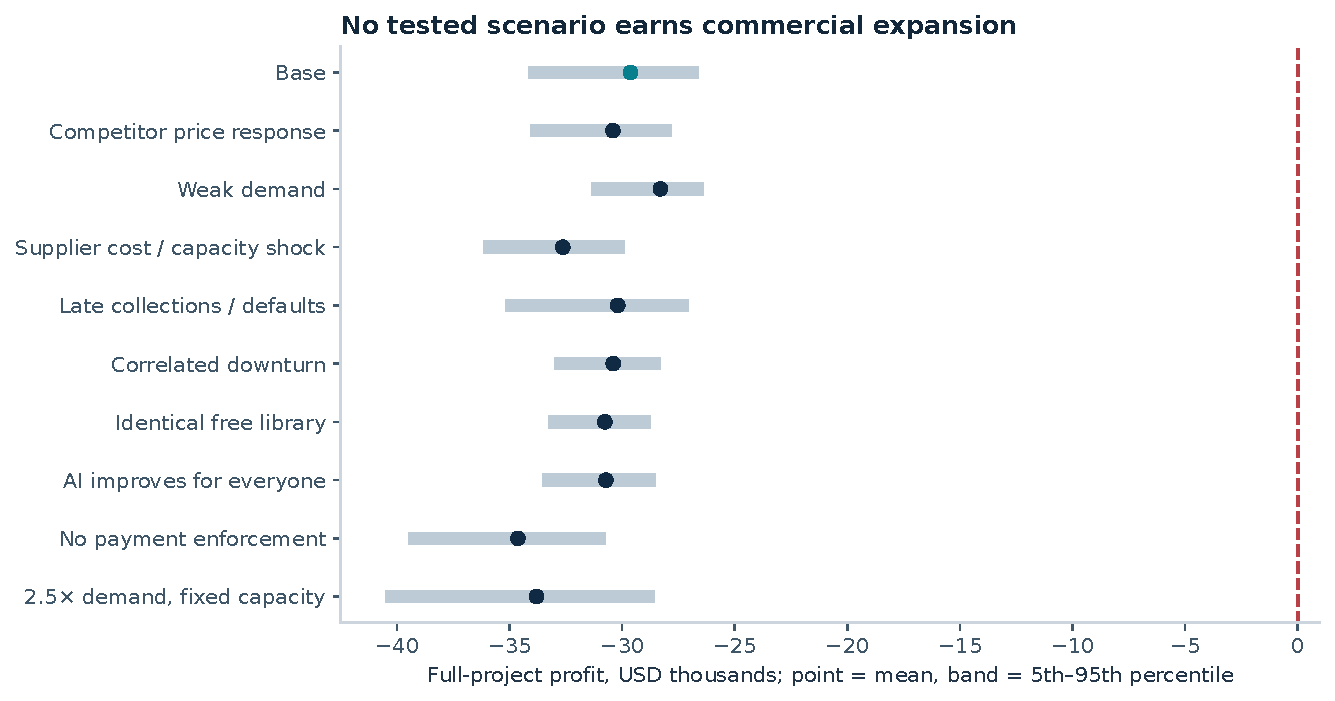
\includegraphics[width=\textwidth]{figures/scenario_results.pdf}
\caption{Mean and 5th--95th percentile profit by scenario. Higher demand creates more acquisition and obligation costs; cheaper AI also strengthens outside options. Neither is assumed to rescue the offering.}
\end{figure}

\subsection{Break-even demand, price, acceptance and cost}
At the observed simulated mix, net revenue including renewals is about US\$1,136 per accepted initial pack, and direct cost including failed work is about US\$735, leaving roughly US\$401 before other campaign costs. Holding that mix fixed gives an optimistic arithmetic break-even requirement of \textbf{82 accepted packs}. The 180-day reserved-capacity ceiling is about 42 orders before failures, sales limits and renewal work. Customer acquisition and support costs would also change with volume; 82 is a diagnostic lower hurdle, not a growth projection.

Holding the approximately eight accepted orders fixed, the mean negotiated price would need to rise from about US\$1,153 to roughly \textbf{US\$4,883} to cover the loss. The development demand response already collapses at much lower posted fees. A fixed discount from a complete instrument's price would therefore be an invalid pricing argument.

Acceptance alone cannot close the gap. Even accepting every currently contracted order at the posted fee, before any variable cost, does not cover the US\$25,700 fixed campaign bill. Eliminating all direct delivery cost still leaves other project costs above net revenue. Eliminating inference charges alone saves only a small fraction of the loss. The constraint is the supported service's complete economic arrangement, not merely a residual model error rate.
